\documentclass[8 pt, twocolumn]{article}

\usepackage[utf8x]{inputenc}
\usepackage{dsfont}
\usepackage{amsthm}
\usepackage{amsfonts}
\usepackage{amssymb}
\usepackage{tensor}
\usepackage{mathtools}
\usepackage[T1]{fontenc}
%\usepackage[spanish]{babel}
\usepackage[cm]{fullpage}
\usepackage{graphicx}
\usepackage{float}
\usepackage{bm}
\usepackage{setspace}
\usepackage{enumitem}
\usepackage{mdwlist}
\usepackage{parskip}
\usepackage{listings}
\usepackage{color}
%\usepackage{epstopdf}
\usepackage{tikz,datatool}
\usepackage{hyperref}
\usepackage{mathabx}

\newcommand{\HRule}{\rule{\linewidth}{0.5mm}}

\AtBeginDocument{
  \let\myThePage\thepage
  \renewcommand{\thepage}{\oldstylenums{\myThePage}}
}

\newcommand{\gra}{$^\text{o}$}
\newcommand{\dif}{\text{d}}
\newcommand{\avg}[1]{\left\langle #1 \right\rangle}
\newcommand{\ket}[1]{\left| #1 \right\rangle}
\newcommand{\bra}[1]{\left\langle #1 \right|}
\newcommand{\bket}[2]{\left\langle #1 \middle| #2 \right\rangle}
\newcommand{\der}[2]{\frac{\text{d} #1}{\text{d} #2}}
\newcommand{\prt}[2]{\frac{\partial #1}{\partial #2}}
\newcommand{\dert}[3]{\frac{\text{d}^#3 #1}{\text{d} #2^#3}}
\newcommand{\prtt}[3]{\frac{\partial^#3 #1}{\partial #2^#3}}
\newcommand{\dl}{\mathcal{L}}
\newcommand{\dha}{\mathcal{H}}
\newcommand{\vol}{\text{vol}}
\renewcommand{\vec}[1]{\pmb{#1}}

\newenvironment{algo}[1]
{  \begin{center}
   \mbox{
       \begin{minipage}{\textwidth}
           \begin{tabbing}
           \settabs
            #1
           \end{tabbing}
        \end{minipage}
    }
    \end{center}
}{}
\newcommand{\settabs}{mmm\=mmm\=mmm\=mmm\=mmm\=mmm\=\kill}

\DeclarePairedDelimiter\ceil{\lceil}{\rceil}
\DeclarePairedDelimiter\floor{\lfloor}{\rfloor}

\definecolor{mygray}{rgb}{0.4,0.4,0.4}
\definecolor{mygreen}{rgb}{0,0.5,0.25}
\definecolor{myorange}{rgb}{1.0,0.4,0}

\definecolor{clock0}{cmyk}{1,0,0,0}
\definecolor{clock1}{cmyk}{1,1,0,0}
\definecolor{clock2}{cmyk}{0,1,0,0}
\definecolor{clock3}{cmyk}{0,1,1,0}
\definecolor{clock4}{cmyk}{1,0,1,0}
\definecolor{clock5}{cmyk}{1,1,1,0}
\definecolor{clock6}{cmyk}{0,0,1,0}
\definecolor{clock7}{cmyk}{0,0,0,0.1}

\begin{document}

\lstset{
language=C++,
basicstyle=\ttfamily\color{black},
commentstyle=\color{mygray}\ttfamily,
frame=single,
numbers=left,
numbersep=5pt,
numberstyle=\tiny\color{mygray}\ttfamily,
keywordstyle=\color{mygreen}\ttfamily,
showspaces=false,
showstringspaces=false,
stringstyle=\color{myorange}\ttfamily,
tabsize=2,
emph={double,uint8_t,uint16_t,uint32_t,uint64_t,int8_t,int16_t,int32_t,int64_t},
emphstyle={\color{blue}\ttfamily}
}

\begin{minipage}[b]{\linewidth}
  \centering
  \Large \textsc{Numerical analysis of the Space Elevator}\\
  ~\\
  \large \textsc{Francisco García Flórez}
\end{minipage}

\section{Abstract}

In this project we are going to study the dynamics of an space elevator, modeled as a number of particles connected by springs under the action of a gravitational potential centered in Earth. Since the equations of motion are not linear, we need to solve them numerically, although, since the solution we are looking for is very specific we can perform the analysis of the movement as small perturbations around an almost static solution.

\section{Theoretical model}

In this section we will lay out the fundamental concepts that are going to be used in the simulation, and introduce the framework in which we will work. Firstly, we will consider the space elevator as an string, physically realized as a finite number of masses attached to each other by springs.

\subsection{Discretized string}

In the following figure we can see a description of the system under consideration:

\begin{figure}[H]
  \begin{center}
    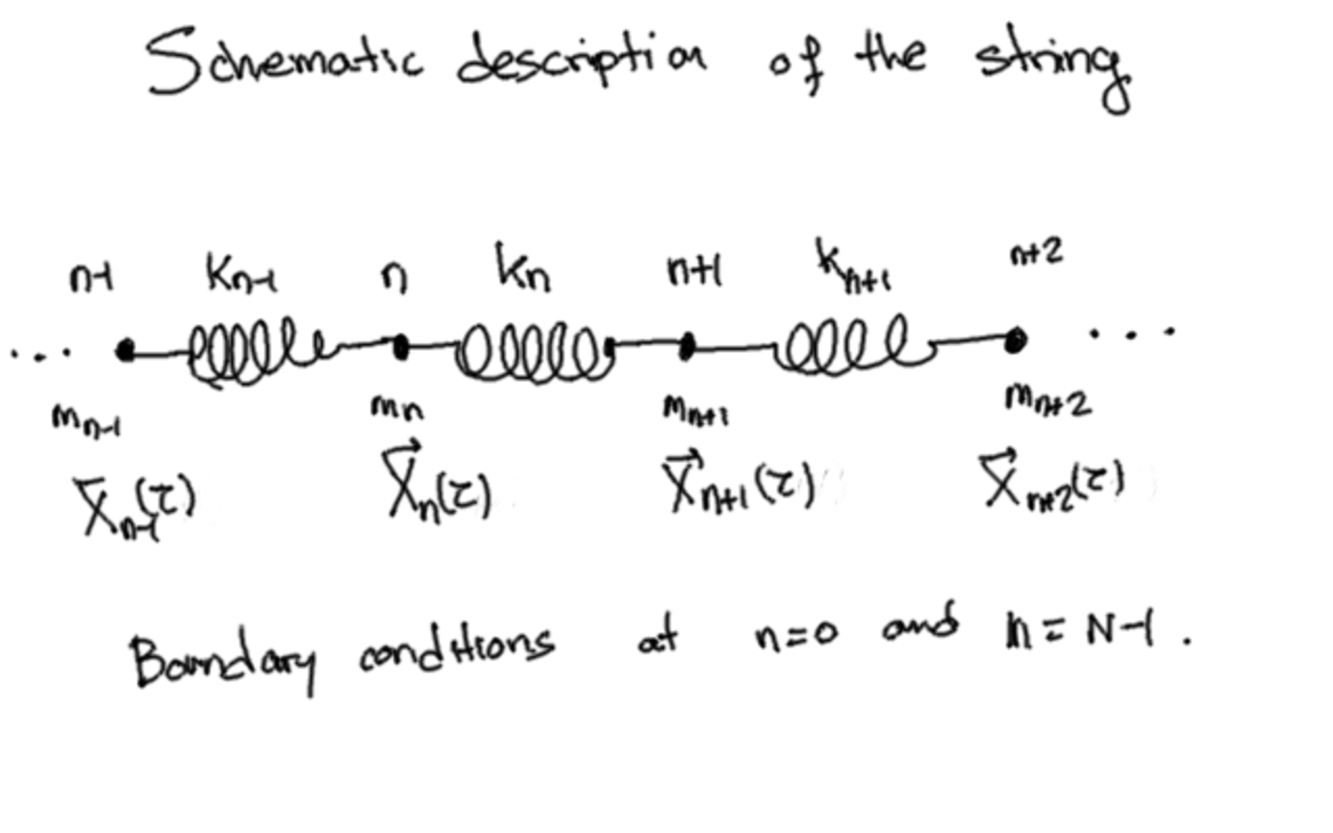
\includegraphics[width=0.5\textwidth]{{../graphs/string}.pdf}
  \end{center}
  \caption{Schematic representation of the discretized string.}
  \label{fig:discrete-string}
\end{figure}

This is clearly a one-dimensional system moving in three dimensions, however in this discretized form we will be considering $N$ particles of different masses coupled by springs under the effect of a spherically symmetric gravitational field. The mass of each particle will be given by $m_n$, and the coupling constant of the spring connecting the particle $n$ and $n+1$ will be $k_n$. Finally, each particle's position will be given by $\vec{X}_n(\tau)$, where $\tau$ is a measure of time, taking the frame of reference in Earth's center of mass.

Since this is a classical mechanics problem, we can write down the Lagrangian and compute $3N$ equations of motion for the string (given by second order differential equations), that afterwards we will compute numerically. We can then split the Lagrangian in three separate contributions:

\begin{equation}
  L = T - V_g - V_s \text{ ,}
\end{equation}

where $T$ is the kinetic term, $V_g$ is the gravitational contribution, and $V_s$ is the spring coupling contribution. It is possible to add other terms to this Lagrangian, that we will discuss later on. Considering the kinetic term first, we have the usual contribution for $N$ particles:

\begin{equation}
  T = \sum_{n=0}^{N-1} \frac{1}{2} m_n \vec{\dot X}^2_n \text{ .}
\end{equation}

For the gravitational contribution, we will consider only Earth's pull, however including other bodies like the Moon wouldn't be a problem, given that we know their trajectories. In principle the full dynamical system would consist of a number of $M$ large bodies under gravitational interactions and the string. Since we are only considering Earth's pull, $V_g$ is as follows:

\begin{equation}
  V_g = \sum_{n=0}^{N-1} \frac{G M m_n}{|\vec{X}_n|} \text{ ,}
\end{equation}

where $G$ is Newton's gravitational constant and $M$ is Earth's mass. Numerically, using kilograms, meters and seconds for these quantities will introduce rounding errors, since $G\sim 10^{-11}$ and $M\sim10^{24}$ in IS units, so we will instead measure $GM$ as a whole, with the following units

$$ GM_{\Earth} = 5.165545706 \cdot 10^{12} \text{ km}^3 \text{ hour}^{-2} \text{ .} $$

This is still a large number, but more manageable. There are also possible generalizations to this term, for example taking into account deviations from spherical shape of the planet, which can produce different contributions in the direction of the north pole compared to the south pole. Continuing with $V_s$, this is the standard spring potential for a number of connected particles, and it reads:

\begin{equation}
  V_s = \sum_{n=0}^{N-1} \frac{1}{2} k_n (\left|\vec{X}_n - \vec{X}_{n+1}\right| - L_0)^2 \text{ ,}
\end{equation}

where $L_0$ is the equilibrium distance of the spring. It is possible to add more terms to this potential as well, like second neighbors interactions, a more realistic potential that introduces non-linearities in the equations of motion or string-breaking terms. Although, we will focus in the small perturbations regime, since having extreme oscillations in the system wouldn't work towards our goal of having an stable space elevator.

\subsection{Equations of motion for the discretized string and boundary conditions}

Now that we have written our Lagrangian, we can proceed to compute the equations of motion using Euler-Lagrange equations:

\begin{equation}
  \der{}{t} \left( \prt{L}{\vec{\dot X}_n} \right) - \prt{L}{\vec{X}_n} = 0 \text{ ,}
\end{equation}

giving us $3N$ second order differential equations that we can solve numerically. Performing this calculations we find:

\begin{multline}
  m_n \vec{\ddot X}_n - \frac{G M m_n}{\vec{X}^2_n} \frac{\vec{X}_n}{|\vec{X}_n|} \\
  +k_{n-1}(\left|\vec{X}_n - \vec{X}_{n-1}\right| - L_0) \frac{\vec{X}_n- \vec{X}_{n-1}}{\left|\vec{X}_n - \vec{X}_{n-1}\right|} \\
  -k_{n}(\left|\vec{X}_{n+1} - \vec{X}_{n}\right| - L_0) \frac{\vec{X}_{n+1}- \vec{X}_{n}}{\left|\vec{X}_{n+1} - \vec{X}_{n}\right|} = 0 ~,~~~\\
  n\neq0 ~,~ n\neq N-1 \text{ .}
\end{multline}

However, this is only valid for the bulk of the string, since $\vec{X}_0$ and $\vec{X}_{N-1}$ are given by the boundary conditions. These conditions may be given by how one particle is connected to the bulk of the string, or they can be fixed to a point in space by a function $\vec{g}(\tau)$. In the former case the equations of motion for the endpoints of the string are

\begin{multline}
  m_0 \vec{\ddot X}_0 - \frac{G M m_0}{\vec{X}^2_0} \frac{\vec{X}_0}{|\vec{X}_0|} \\
  -k_{0}(\left|\vec{X}_{1} - \vec{X}_{0}\right| - L_0) \frac{\vec{X}_{1}- \vec{X}_{0}}{\left|\vec{X}_{1} - \vec{X}_{0}\right|} = 0
\end{multline}

\begin{multline}\label{eq:spacebound}
  m_{N-1} \vec{\ddot X}_{N-1} - \frac{G M m_{N-1}}{\vec{X}^2_{N-1}} \frac{\vec{X}_{N-1}}{|\vec{X}_{N-1}|} \\
  +k_{N-2}(\left|\vec{X}_{N-1} - \vec{X}_{N-2}\right| - L_0) \frac{\vec{X}_{N-1}- \vec{X}_{N-2}}{\left|\vec{X}_{N-1} - \vec{X}_{N-2}\right|} = 0 \text{ .}
\end{multline}

However, we won't be applying these boundary conditions at the same time, since finding a stable solution without direct interactions with the surface of Earth is rather difficult. Instead, we will leave the space endpoint free, using (\ref{eq:spacebound}) only, and the following for Earth's endpoint (``anchor'' in the following):

\begin{multline}
  \vec{X}_0(\tau) = \\ R_\Earth
    \begin{pmatrix}
      \cos(\omega_\Earth \tau) \cos(\theta) + \sin(\omega_\Earth \tau) \sin(\theta) \\
      -\cos(\omega_\Earth \tau) \sin(\phi) \sin(\theta) + \sin(\omega_\Earth \tau) \sin(\phi) \cos(\theta) \\
      \cos(\omega_\Earth \tau) \cos(\phi) \sin(\theta) - \sin(\omega_\Earth \tau) \cos(\phi) \cos(\theta)
    \end{pmatrix}
  \text{ ,}
\end{multline}

where $R_\Earth$ is Earth's radius, $\omega_\Earth$ is Earth's rotation angular velocity and the angles $\phi$ and $\theta$ is the location of the elevator anchor on the surface, as latitude and longitude. Usually we will consider $\phi = \theta = 0$, since having the anchor at the equator is the most stable solution, but we can also analyze the effect of a small separation from that point in the motion of the cable.

Physically, this boundary condition means that we are pulling from the cable at the surface, keeping it in place instead of being sling-shot away from the planet. Since we are assuming this force is strong enough, we will set $m_{N-1}$ to a special value. This endpoint will be called counter-weight (``CW'', from now on) for this very reason, since we will consider a much larger mass for it than for the rest of the string.

Finally, once we have our equations of motion as second order differential equations, we need to convert them to a system of $6N$ first order differential equations that we can then numerically solve.

\subsection{Initial conditions and mass profile}

Finding an stable solution for this system is not an easy task, since small perturbations to the parameters can significantly affect the motion. An stable solution is schematically represented in Figure \ref{fig:stable-sol}.

\begin{figure}[H]
  \begin{center}
    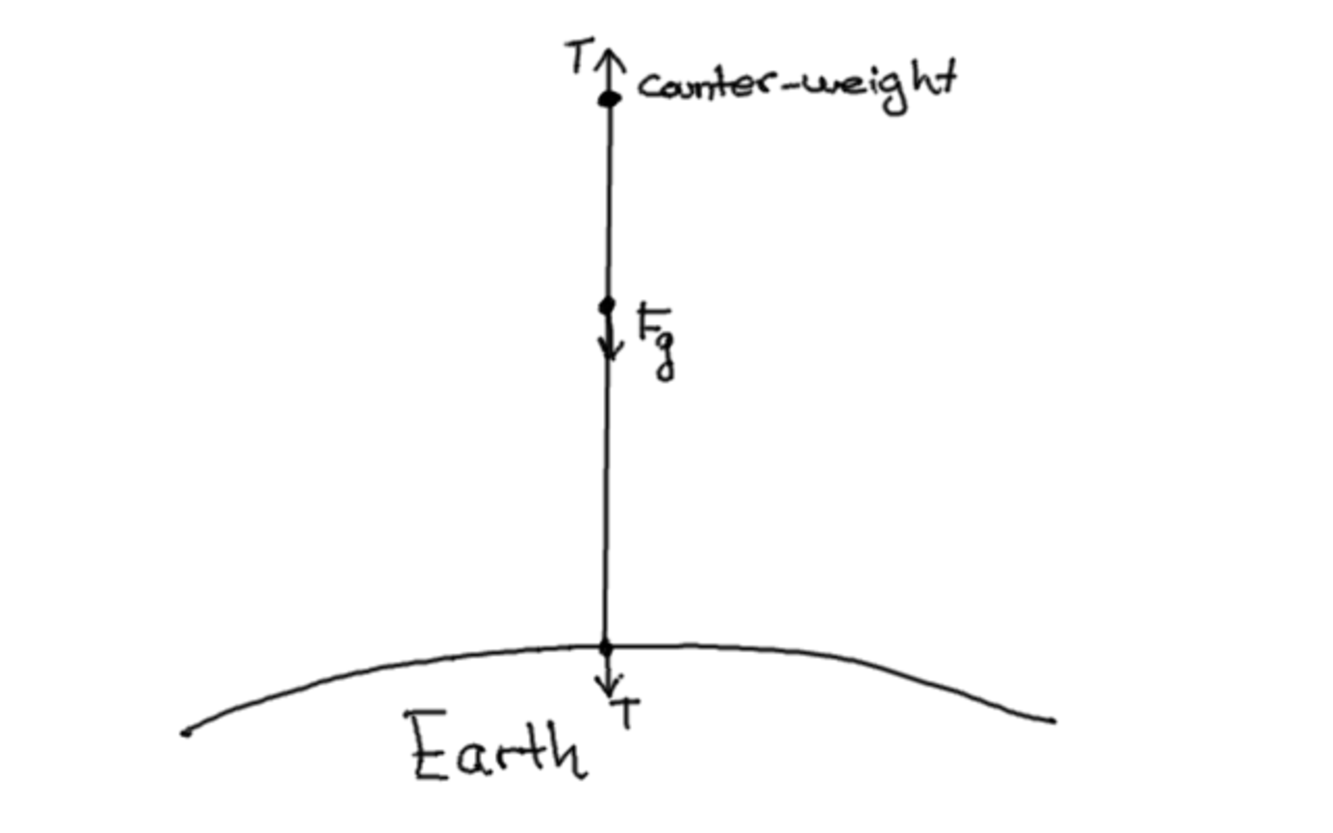
\includegraphics[width=0.5\textwidth]{{../graphs/elevator}.pdf}
  \end{center}
  \caption{Schematic representation of a stable solution.}
  \label{fig:stable-sol}
\end{figure}

In this figure we can see how the outwards tension produced by the rotational motion has to be compensated by the gravitational force downwards and the tension at the anchor, however this compensation will never be perfect, since it is not possible to have a totally static solution without any longitudinal or transversal modes whatsoever.

Another obvious problem we will have to deal with is the fact that we need each point of the string to follow a circular orbit, however we know from undergraduate orbital mechanics that the velocity of a body in a circular orbit of radius $R$ is constant and given by

$$ v_{\text{circular}} = \sqrt{\frac{GM}{R}} \text{ ,} $$

while the tangential velocity of a body rotating with angular velocity $\omega$ is

$$ v_{\text{rotation}} = \omega R \text{ ,} $$

where $R$ is the distance to the axis of rotation. Obviously, for the space elevator these two velocities will only be equal at the geosynchronous orbit, so there will be longitudinal modes moving along the string forcing it to stay as close to the stable solution as possible. In the following section we will analyze such modes.

A final question we need to consider is the mass profile of the string, or $m_n$ and $k_n$ as functions of $n$. To make the definition easier, we will consider the string as an one-dimensional continuous object $\vec{X}(\tau,\sigma)$, where now $\sigma \in [0, 1]$ and for the stable solution represented in Figure \ref{fig:stable-sol} it will look like $|\vec{X}(\tau,\sigma)| = R_\Earth + R \sigma$, where $R$ is the length of the cable. This way, $m_n$ will be given as:

\begin{equation}
  m_n = m(n\Delta\sigma) ~, ~~~ m(\sigma) = \tilde m_0 f(\sigma) \text{ ,}
\end{equation}

Since our initial condition will always be this static solution (``straight string'', from now on) $\sigma$ can be easily computed for each node. This $f(x)$ function will be a second order polynomial that we will also use to compute $k_n$, and is given in general by:

\begin{equation}
  f(x) = \alpha + \beta x + \gamma x^2 = \frac{1-(b-a)c - a}{c(c-1)} (x^2-x)+(b-a)x +a \text{ ,}
\end{equation}

where the coefficients have been fixed by imposing $f(0) = a$, $f(1) = b$ and $f'(c)=0$. We choose this function to match numerical results from [1], where an optimal mass and spring coupling profiles are given.

\section{Results}

\subsection{Simulation settings}

Before stating the initial conditions of the simulation, we need to configure several parameters of the simulation itself. First, as we mentioned before we will use kilometers and hours as units of length and time, and standard kilograms as mass. With this, we are only going to consider an space elevator on Earth, so the gravitational potential will have as a constant

\begin{equation}
  GM_{\Earth} = 5.165545706 \cdot 10^{12} \text{ km}^3 \text{ hour}^{-2}  \text{ ,}
\end{equation}

as we mentioned before. Other constants specified for Earth:

\begin{equation}
  \begin{dcases*}
    R_\Earth = 6731 \text{ km} \\
    \omega_\Earth = 0.2617993877991494 \text{ hour}^{-1} \\
    \phi = \theta = 0
  \end{dcases*} \text{ .}
\end{equation}

We need to specify as well for how many hours the simulation will run, and how many steps are calculated. In a more technical note, we will be using [2], a library written in C++ for integration of first order systems of ordinary differential equations.

\subsection{Initial configuration}

Now, as we mentioned earlier, we will start from a straight string configuration with Earth's endpoint situated on the anchor, and constant angular velocity in the same direction of Earth's rotation. After several simulations, we found the right values for the initial conditions so that we find an stable solution, summarized in the following:

\begin{equation}
  \begin{dcases*}
    N = 100 \\
    R = 10^5 \text{ km} \\
    \alpha = 0.85 \\
    L_0 = \alpha R/N \sim 850 \text{ km} \\
    Y_0 = 7.7 \cdot 10^{4} \text{ km}^{-1} \text{ kg hour}^{-2} \\
    a = 0.4 \\
    b = 0.7 \\
    c = 0.6 \\
    \tilde m_0 = 12 \text{ kg km}^{-1} L_0 \sim 10.2 \cdot 10^3 \text{ kg} \\
    \tilde k_0 = Y_0 L_0 \\
    m_{N-1} = 10^6 \text{ kg} \\
  \end{dcases*}
  \text{ .}
\end{equation}

Here $a$, $b$ and $c$ are the constants that specify $f(x)$ and thus the mass and spring couplings profile. $Y_0$ is Young's modulus, thus giving $k_n$. We are only considering a hundred nodes on the string due to technical limitations, as the number of calculations increases significantly with $N$. The length of the cable is an interesting parameter, since we can adjust it so that the center of mass of the string is above or below the geosynchronous orbit, and thus the cable would tend to get sling-shot or fall to earth.

Another relevant parameter is $\alpha$, since we need to take into account that the string will stretch, and it can fall to the ground in the first time steps if the string is at equilibrium. CW's mass also significantly affects the motion, since a large mass at the endpoint will greatly stabilize the solution, by establishing a clear straight line from where the string will deviate.

Although, this initial configuration is suited for a numerical simulation, since it solves problems found when the elevator is already at the straight solution. In reality, engineering a method of deployment requires a completely different approach, since it would probably involve a slow construction in space, directly at the counter-weight, from where an equally slow deployment to the ground would take place. Of course, it is possible to simulate this situation, however in this project we are interested on the orbital mechanics once it has been placed.

\subsection{Counter-Weight motion and oscillation modes}

Even though for us the CW is only a node more massive than the rest, in reality that would be the place where spaceships or space stations would be located, and mainly from where every travel would start. Because of this, its motion is highly relevant from the engineering point of view, since too disruptive perturbations from the equilibrium would make trajectory prediction unreliable.

Therefore, in this section we compute the motion of only this node in the string, but focusing in the longitudinal motion, normal to the surface of the planet. This distance corresponds with $|\vec{X}_{N-1}(\tau)|$, and it is plotted in Figure \ref{fig:CW-motion}:

\begin{figure}[H]
  \begin{center}
    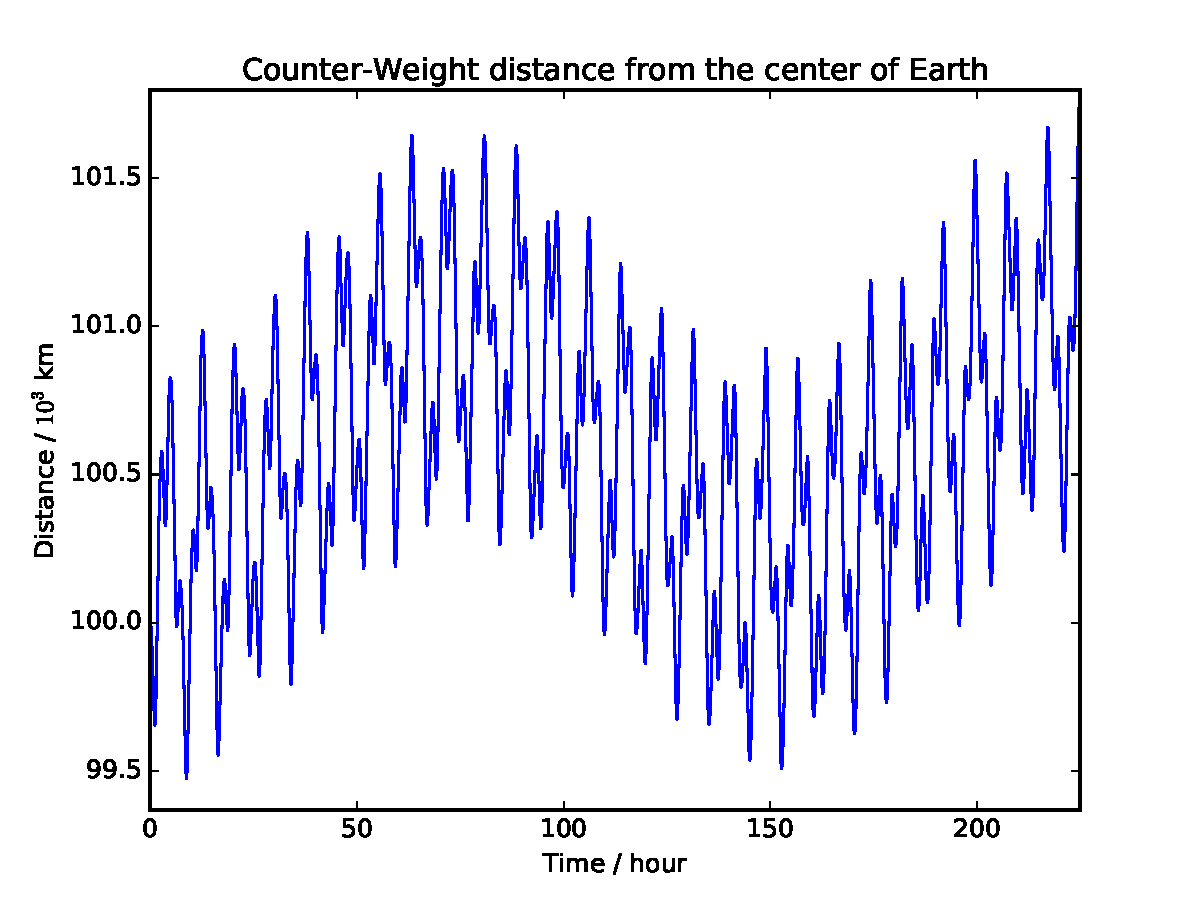
\includegraphics[width=0.5\textwidth]{{../graphs/CW-dist}.pdf}
  \end{center}
  \caption{Longitudinal motion of the CW.}
  \label{fig:CW-motion}
\end{figure}

Here we can make several remarks. First of all, we have oscillatory motion both at high and low frequencies, and even if this plot covers $\sim220$ hours of simulation, we can notice that it's increasing, hinting at another even lower frequency mode. Now, the scale in the y axis is $10^3$ km, so the CW moves up and down over a distance of $2\cdot10^3$ km. This amount is negligible compared to the length of the string, however it could be desirable to decrease it even more.

We can analyze this plot in frequency space by Fourier transforming and studying the frequency spectrum that we can see in Figure \ref{fig:CW-modes}:

\begin{figure}[H]
  \begin{center}
    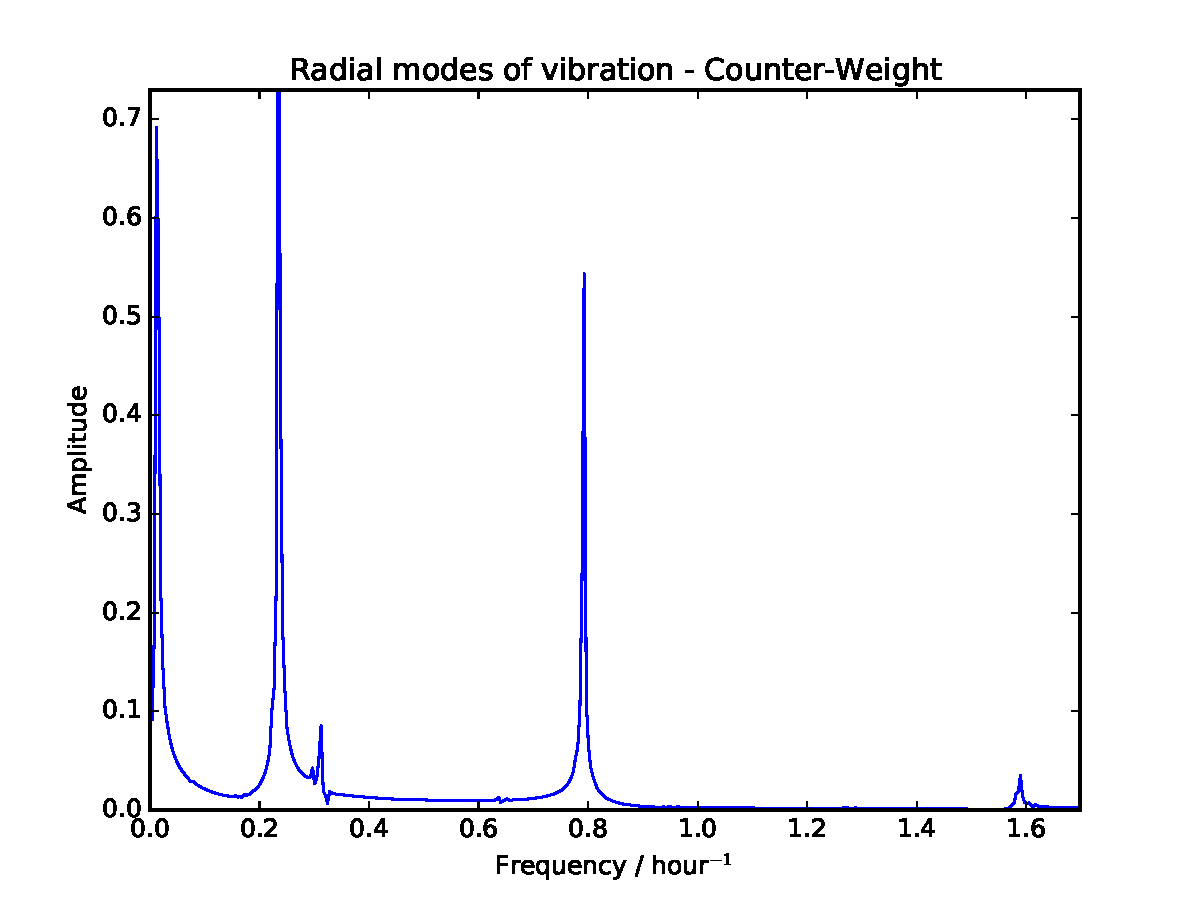
\includegraphics[width=0.5\textwidth]{{../graphs/CW-modes}.pdf}
  \end{center}
  \caption{Frequency spectrum of the longitudinal modes of the CW.}
  \label{fig:CW-modes}
\end{figure}

Since we don't have enough time steps, we can't probe high frequencies however we do find good resolution at low frequencies. Of course, we were expecting sharp and independently realized oscillation modes because of our approximation about the string couplings, as we know the solution to the wave equation is a sum of oscillatory modes.

It is also clear that ultra low frequencies are compressed into the first point, unresolved. However it is clearly visible that significant contribution at frequency $\sim4$ hours, and another one at $\sim75$ minutes.

\subsection{Length perturbations}

Related to the previous section, we can compute the length of the string as a function of time. Even though the following plot will look extremely similar to Figure \ref{fig:CW-motion}, in this case we are also considering normal perturbations. As we can see in the following Figure:

\begin{figure}[H]
  \begin{center}
    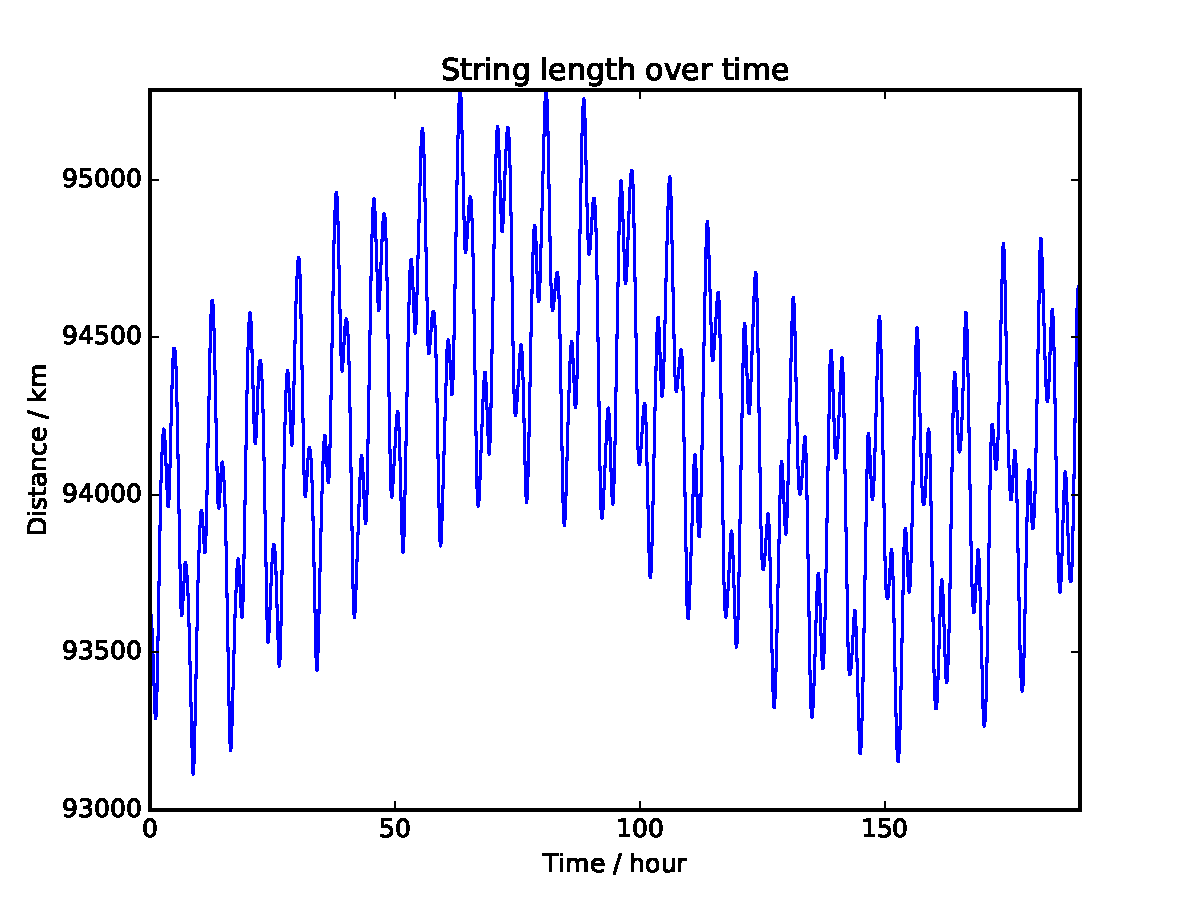
\includegraphics[width=0.5\textwidth]{{../graphs/length}.pdf}
  \end{center}
  \caption{Length of the string as a function of time.}
  \label{fig:length-evol}
\end{figure}

This fact is a sign of a good configuration, since it means that normal modes are almost nonexistent, while still keeping a motion close to the straight solution. Another significant remark about the length, is that it is related to the tension applied over the string. In Figure \ref{fig:avg-sep} we can visualize at what points the string is more stretched:

\begin{figure}[H]
  \begin{center}
    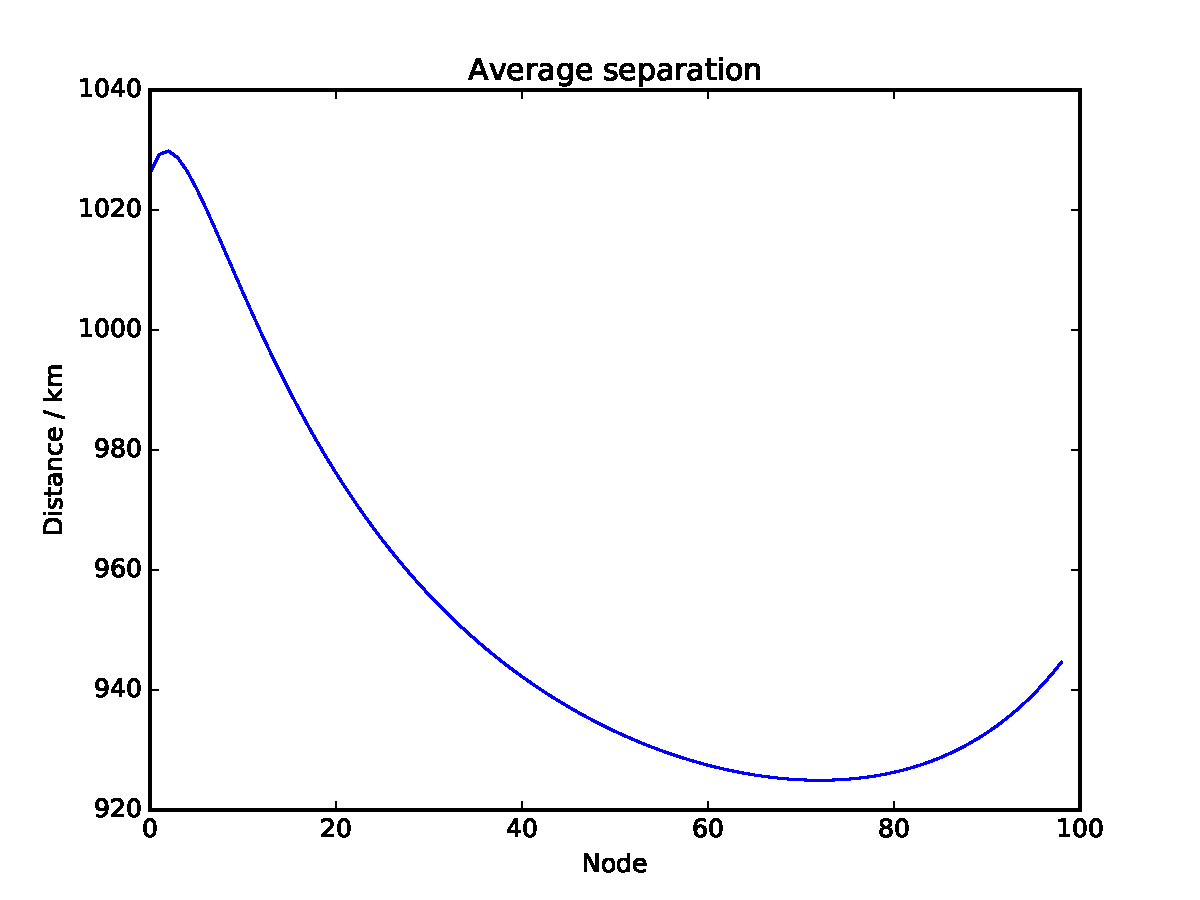
\includegraphics[width=0.5\textwidth]{{../graphs/stretch}.pdf}
  \end{center}
  \caption{Average separation between nodes.}
  \label{fig:avg-sep}
\end{figure}

Recalling that the length of the string is around a hundred thousand kilometers, it is easy approximate where each node is located in terms of altitude. Remember as well that the geosynchronous orbit is located at height $\sim40\cdot10^3$ km, so we expect a change in the plot for nodes above and below this point, as we indeed see above. Also as we were expecting, near the surface the separation peaks, so the engineering involved in building this anchor would be a delicate problem.

This is not, however, the end of the story. The force is not linearly related to the separation because of the different spring coupling constants, so in Figure \ref{fig:avg-force} we can see the tension density:

\begin{figure}[H]
  \begin{center}
    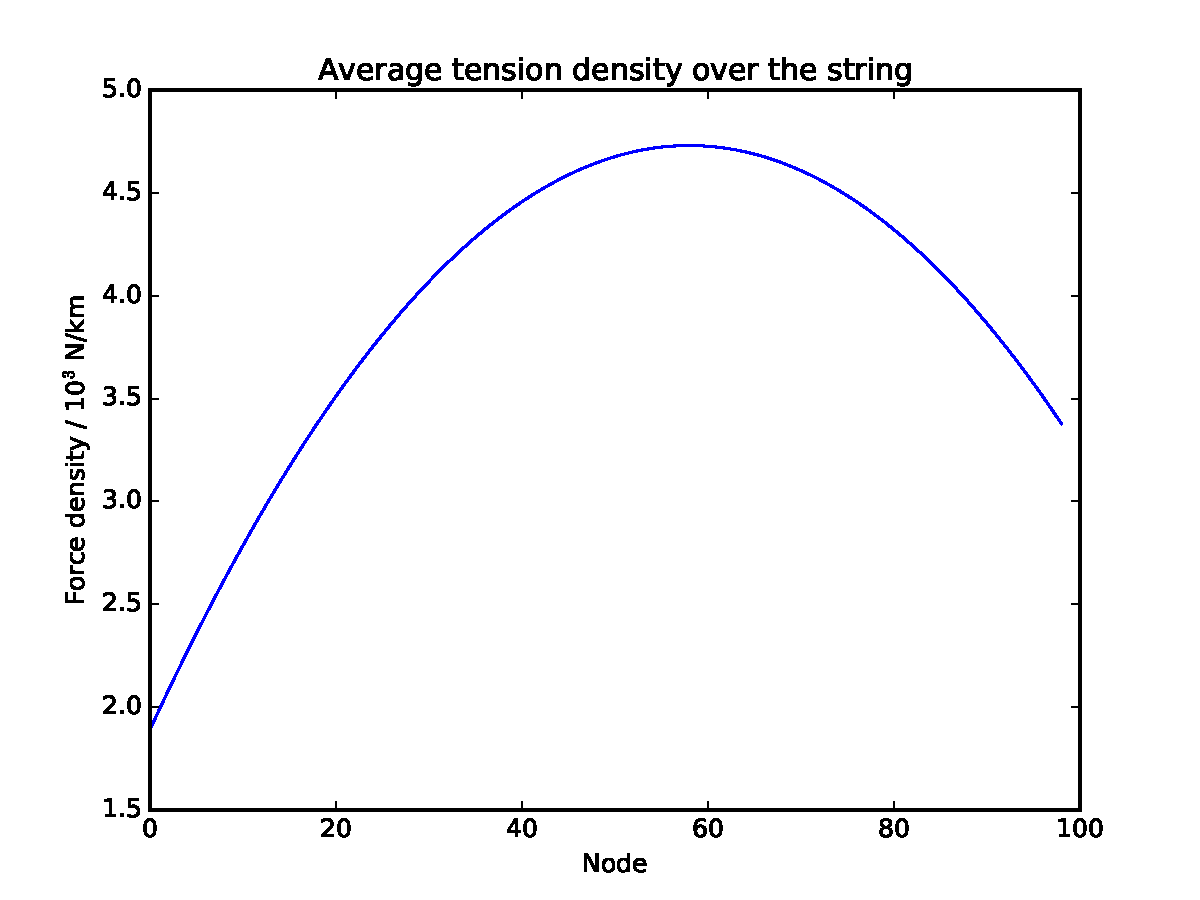
\includegraphics[width=0.5\textwidth]{{../graphs/force}.pdf}
  \end{center}
  \caption{Average spring tension density between nodes.}
  \label{fig:avg-force}
\end{figure}

Now we can clearly see why in Figure \ref{fig:avg-sep} there is a valley around node 70, because by choosing the parameter $c=0.6$ we are making the string stronger at that point. In principle we could choose completely different mass and couplings profiles, for the sake of reality we assume that both share the same shape, and thus at this peak the elevator is the most massive. Physically we can interpret this as having a material of constant density but thicker around this point.

It would be of course desirable that the tension is uniformly distributed along the string, and finding the right profile would be a very interesting analytical and numerical problem. It is possible to use our program for this purpose, by running several simulations and varying the profile until the force is approximately uniform, however we won't focus on this.

\subsection{Normal perturbations from straight solution}

In this section we will be focusing on the perturbations tangential to the straight solution, however we need to introduce some transformations to be able to extract this information. Since the motion is fairly simple, only in the X-Y plane and around the planet, we will take $\vec{X}_n(\tau)$ and transform it to a new basis where tangential modes will be contained to the Y axis, and longitudinal modes to the X axis.

We achieve this by making a rotation for each simulation step $\tau$, of an angle given by the CW and the anchor. In Figure \ref{fig:rotation} an scheme of this transformation is shown, and it is performed at each simulation step.

\begin{figure}[H]
  \begin{center}
    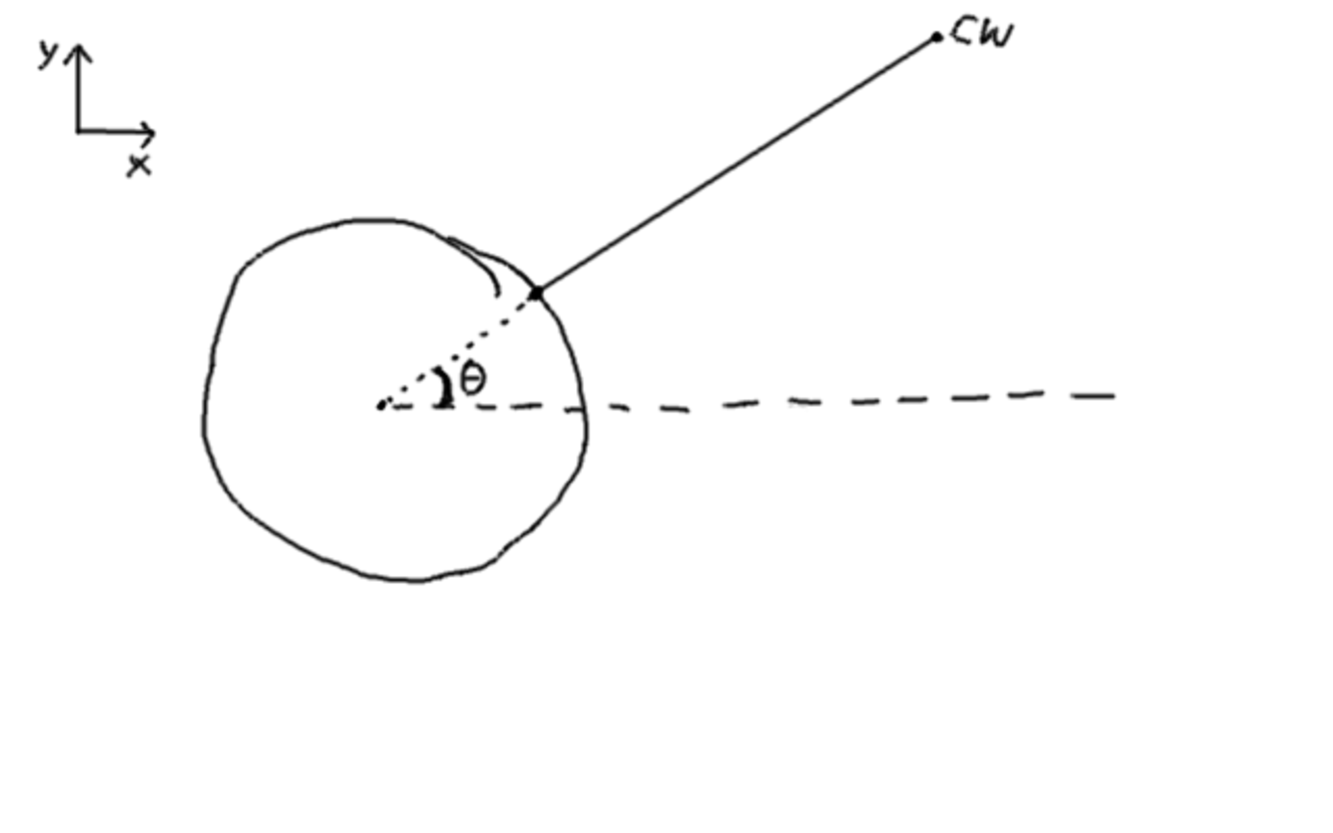
\includegraphics[width=0.5\textwidth]{{../graphs/rotation}.pdf}
  \end{center}
  \caption{Schematic representation of the rotation.}
  \label{fig:rotation}
\end{figure}

The angle $\theta$ is easily computed by displacing the CW position to the frame of reference $\vec{X}_{CW}-\vec{X}_0$ and then computing $\theta=\arctan(y/x)$. After applying this rotation to the whole string we find $\vec{\tilde X}_n(\tau)$ in the new coordinates, and in Figure \ref{fig:tan-perts} we can see the result.

\begin{figure}[H]
  \begin{center}
    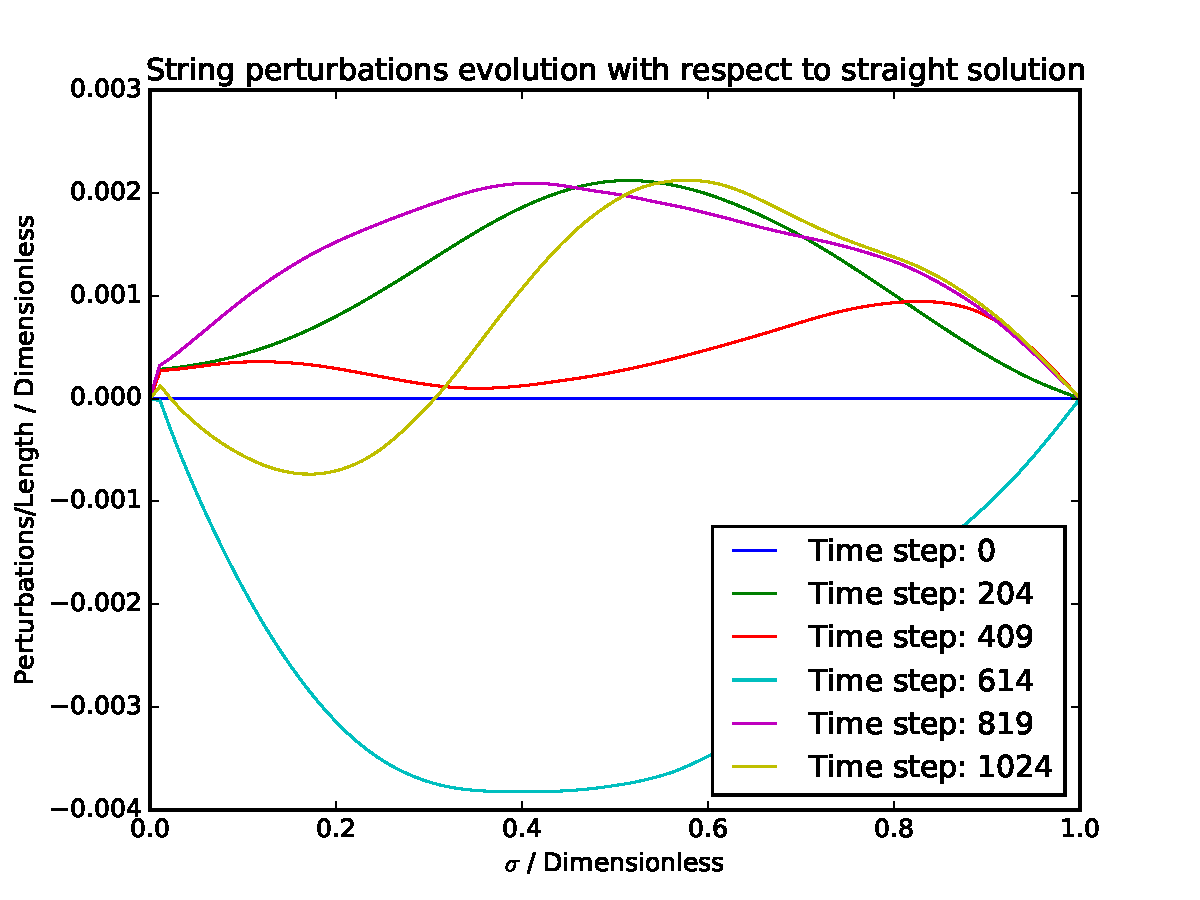
\includegraphics[width=0.5\textwidth]{{../graphs/normal-perts}.pdf}
  \end{center}
  \caption{Tangential perturbations divided by length, at different time steps.}
  \label{fig:tan-perts}
\end{figure}

Here we are using the parameter $\sigma$ instead of node number, since this is a better representation of the dynamics. In the Y axis perturbations are plotted, and as we can see they are almost negligible, less than 0.5\% of the length of the elevator, in real space that amounts to $\sim500$ km. Of course, the importance of these perturbations is significant, since anything running up or down along the elevator will be subject to forces derived from this motion.

We can represent this motion in a different way, by means of a temperature plot as we can see in Figure \ref{fig:temp-perts}.

\begin{figure}[H]
  \begin{center}
    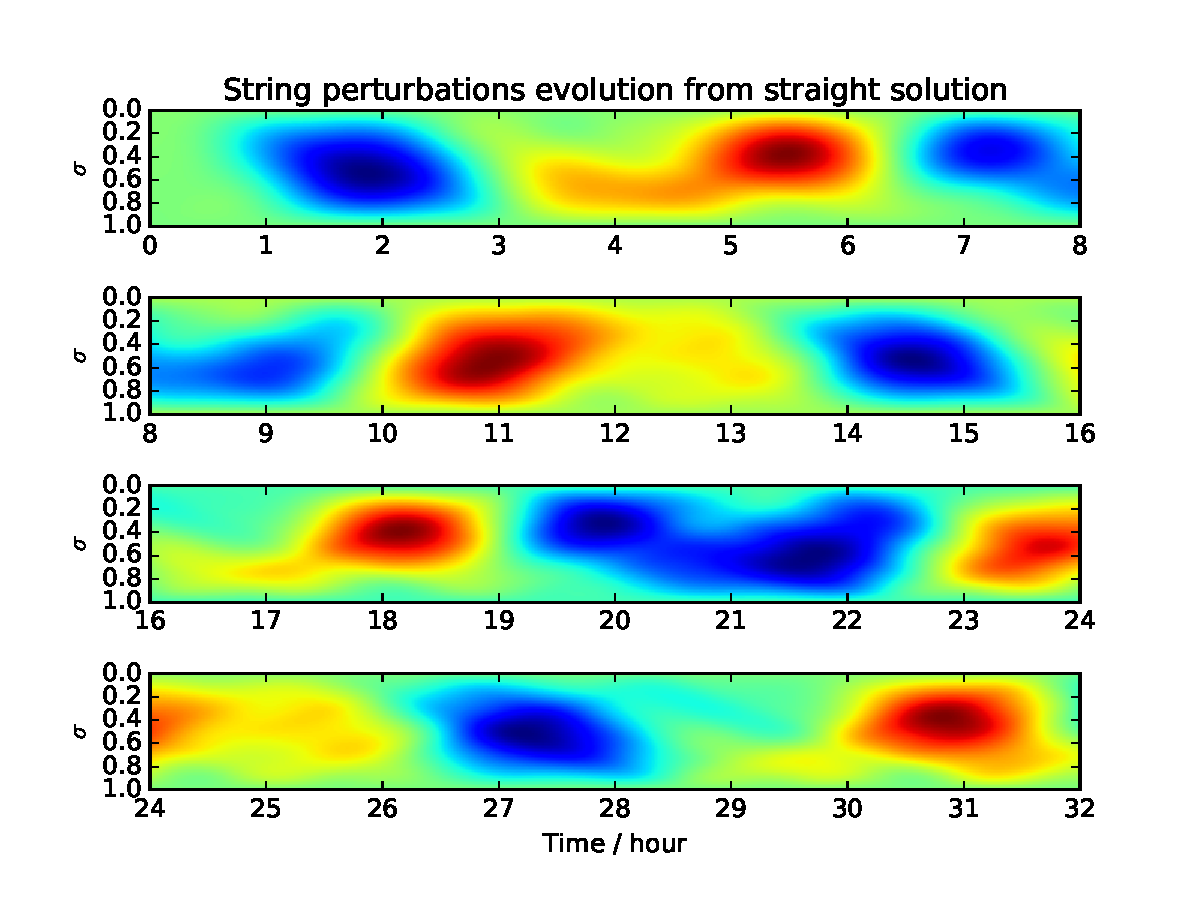
\includegraphics[width=0.55\textwidth]{{../graphs/straight-perts}.pdf}
  \end{center}
  \caption{Temperature plot of tangential perturbations from the straight solution.}
  \label{fig:temp-perts}
\end{figure}

In this case we can't represent the whole simulation, but we can clearly see the periodicity of the perturbations. As before, a mode of frequency $\sim14^{-1}$ hours is clearly visible, as well as others of higher frequency $\sim6^{-1}$ hours. Now, another detail we can extract from this plot, in the first perturbation we can clearly see that it takes $\sim2.5$ hours to propagate a perturbation in the surface to the CW, a sound speed of $c_s\sim40\cdot10^3$ km hour$^{-1}$.

Comparing this value with [1], we see that longitudinal perturbations propagate at $\sim100\cdot10^3$ km hour$^{-1}$ much faster than our tangential modes. In the following plot we represent the average deviance from straightness at each time step, and it's clear that the pattern is completely different to what we saw for longitudinal perturbations.

\section{Extensions to this model}

Due to time limits, we weren't able to include as many effects as it would be possible in the simulation. Nevertheless, in this section we will summarize a few of these.

\subsection{General relativity}

Even though our system has been modeled as a discretized string, a more analytically-fitted approach would be to consider a field $X^\mu(\tau, \sigma)$ defined over a 2-manifold satisfying the following action:

\begin{equation}
  S_p = T \int \dif \tau \dif \sigma ~ \partial_\alpha X^\mu \partial^\alpha X_\mu \text{ , }~~ \partial_\alpha = \left( \prt{}{\tau}, \prt{}{\sigma} \right) \text{ ,}
\end{equation}

also known as Polyakov's action. This is the fundamental equation in bosonic string theory, however it can be perfectly used in our system. Of course, we would need to adapt this action to our needs, but there is one change specially easy to introduce: the effects of gravity in general relativity. This situation is know in string theory as a \emph{curved background}, but in our case it's much more simple. The new action reads:

\begin{equation}
  S = T \int \dif \tau \dif \sigma ~ \partial_\alpha X^\mu \partial^\alpha X^\nu G_{\mu\nu}(X) \text{ ,}
\end{equation}

Where this $G_{\mu\nu}(X)$ would be the space-time metric where the string is moving. Since in this case we are only considering one source of spherically symmetric gravitational potential, it would be given by the Schwarzschild metric:

\begin{multline}
  c^2 {d \tau}^{2} = \\\left(1 - \frac{r_s}{r} \right) c^2 dt^2 - \left(1-\frac{r_s}{r}\right)^{-1} dr^2 - r^2 \left(d\theta^2 + \sin^2\theta \, d\varphi^2\right) \text{ .}
\end{multline}

Variations to the motion of the string introduced by this change would be extremely negligible, however it is widely known that GPS satellites work on time scales in which they aren't, and general relativity needs to be considered. In our case, if we wanted to synchronize high precision clocks along the string correctly, then nanosecond deviation wouldn't be negligible, and thus general relativity has to be considered.

\subsection{Other bodies}

A different approach would be to consider perturbations due to Moon's gravitational pull. For this we have two possibilities, either we consider both Earth and Moon as a gravitationally bounded system, fundamentally being a 2-body problem, or we fix Moon's motion to an approximation of the orbit it follows and introduce another term in the Lagrangian, that would look like

\begin{equation}
  V^\Moon_g = \sum_{n=0}^{N-1} \frac{G M_\Moon m_n}{|\vec{X}_n-\vec{R}_\Moon|} \text{ ,}
\end{equation}

where $\vec{R}_\Moon(\tau)$ is a fixed function approximating the position of the Moon.

\subsection{Deviations from spherical symmetry in the gravitational potential}

Lastly, another trivial generalization we may consider is the introduction of extra terms to the gravitational potential of the Earth, given by a multipole expansion of the full potential. As explained before, $V_g$ seen as the first term of this multipole expansion can be seen as concentrating the mass of the planet in a point. The next term, called quadrupole, can be computed and it is given by

\begin{equation}
  V^{(2)}_g = \frac{G}{|\mathbf{x}|} \int_V \dif m(\mathbf{r}) ~ \left(\frac{r}{|\mathbf{x}|}\right)^2 \frac {3 \cos^2 \theta - 1}{2} \text{ .}
\end{equation}

In this case we are considering a position-dependent density for the planet, but it can be simplified in the final model.

\section{Conclusions}

Concluding, we have successfully solved the motion of the space elevator in a physically interesting situation by numerical means, and found a stable solution that can be improved to meet the engineering requirements that a project of this extreme complexity would have.

We have also summarized how can this model be extended, and gave a few ideas as to how a more physical situation could be modeled. For further information in this topic [1] is a great source.

\section{References}

\begin{enumerate}[label={[\arabic*]}]
  \item Lang, David. \emph{Space Elevator, Dynamics Reference Manual, Section 1}.
  \item K. Ahnert and M. Mulansky, \emph{Odeint - Solving Ordinary Differential Equations in C++}, AIP Conf. Proc. 1389, pp. 1586-1589 (2011); doi:http://dx.doi.org/10.1063/1.3637934
\end{enumerate}

\end{document}
